\documentclass[12pt]{article}
\usepackage[utf8]{inputenc}
\usepackage[english]{babel}
\usepackage{graphicx}
\usepackage{float}


\setlength{\oddsidemargin}{0in}
\setlength{\evensidemargin}{0in}
\setlength{\textwidth}{6.5in}
\setlength{\topmargin}{-.3in}
\setlength{\textheight}{9in}
\setlength{\parskip}{1em}

% \pagestyle{empty}
\graphicspath{ {images/} }
% ___________________________________________________________________

\begin{document}

\begingroup  
  \centering
  \large Report: Experiments on $\alpha$ updates \par
  \large Arijus Pleska \par
\endgroup
% ___________________________________________________________________

\par This report assesses some experiments performed on reproducing $\alpha$ parameters used in a generative data process. Note that the report is structures in the following sections: 1) defining the experiment settings; 2) assessing the experiment results; 3) settings some questions to be discussed during next meeting.
% ___________________________________________________________________

\section*{The Experiment Settings}

\par The intention of the carried experiments is to identify the optimal settings for the Metropolis--Hastings algorithm application. 
To start with, I have generated a synthetic corpus; the parameters used in the corpus generation will allow to assess the performance achieved in the experiments. The corpus generation parameters are set as follows:
\begin{itemize}
	\item The number of topics: K = 2;
	\item The number of documents (time-slices): T = 20;
	\item The size of vocabulary: V = 10;
	\item The number of words per document t: $N_t \sim \mbox{Pois}(\lambda),\quad \lambda = 1000$.
\end{itemize}
Further, to consider the initial settings of $\alpha_k$ development over documents, $\alpha_0$ is a sine curve and $\alpha_1$ is a cosine curve; the corresponding \textit{softmax} expressions of the curves are illustrated in Figure 1 below.
\begin{figure}[H]
  \centering
  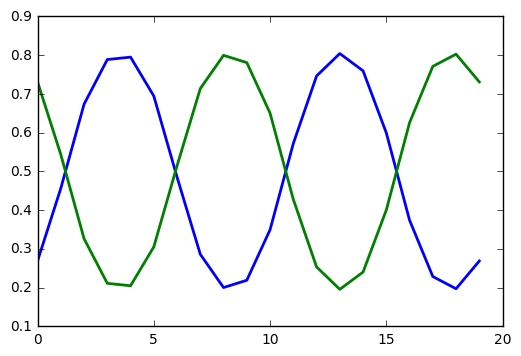
\includegraphics[width=0.5\textwidth]{alpha_initial}
  \caption{The values of $\mu$ used in the generative process.}
  \label{fig:mu}
\end{figure}
Speaking of $\beta$, it was initially predefined and kept constant throughout the dynamic generative process; $\beta$ is illustrated in Figure 2 below.
\begin{figure}[H]
  \centering
  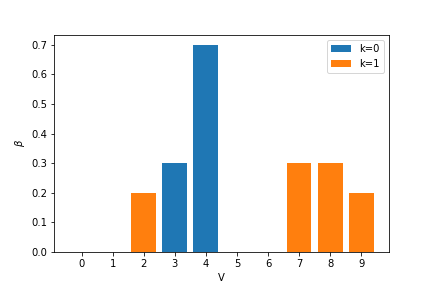
\includegraphics[width=0.5\textwidth]{beta_initial}
  \caption{The values of $\beta$ used in the generative process.}
  \label{fig:beta}
\end{figure}
Note that the latter $\beta$ values were applied to the autoregressive topic model for the $\alpha$ update experiments.
% ___________________________________________________________________

\section*{The experiment results}

\par

% ___________________________________________________________________
\subsection*{Current Stage}

% - Data and model settings
% -- Synthetic data set
% -- Parameters initialisation
% --- Number of topics
% --- Initial alphas and betas
% ---- Variance

\par During the experiment, I have used the following settings:
\begin{itemize}
\item The synthetic data has been created by inducing the previously implemented dynamic topic modelling (DNT) generative process:
\begin{itemize}
\item The number of documents: $|\mbox{D}|\approx6000$;
\item The size of the vocabulary: $|\mbox{V}|\approx2000$;
\item The number of words per document: $\mbox{N}_d\approx20$,\quad$\forall d \in \mbox{D}$;
\item Instead of intensity values, it is assumed that the document dictionaries contain word counts. For example, $d_{111}=\{v_{20}:15, v_{40}:5\}$. 
\end{itemize}
\item The number of topics: $K=10$;
\item The number of time-slices: $T=50$;
\item The alpha at $t=0$: $\alpha_0 \sim \mathcal{N}(\mu_0, \sigma^2_0I),\quad \mu_0 = 0.1,\quad\sigma_0^2 = 0.2$;
\item The alphas at $t>0$: $\alpha_t \sim \mathcal{N}(\alpha_{t-1}, \sigma^2I), \quad\sigma^2 = 0.1$;
\item The candidate alphas: $\alpha'_t \sim \mathcal{N}(\alpha_{t}, \delta^2I), \quad\delta^2 = 2$; 
\item The acceptance rate: $r_t=\min(1,p(\alpha'_t)/p(\alpha_t))$;
\item The probability of the state: $p(\alpha_t)=p(\alpha_{t} | \alpha_{t-1})\cdot p(\alpha_{t+1} | \alpha_{t})\cdot \pi(\alpha_t)$, where $\pi$ is a mapping to the mean parameterisation;
\end{itemize}

The rationale of the implementation follows the following principle: $\alpha_t$ is set to $\alpha'_t$ on the successful `toss' based on $r_t$. Also, the variances are tuned to obtain $r_t\approx30\%$.

\subsection*{Issues}
\par My uncertainties with the proposed solution are the following:
\begin{itemize}
\item The estimation of $p(\alpha_t)$:
\begin{itemize}
\item The third term of the expression, $\pi(\alpha_t)$, represents the topic distribution in documents in time-slice $t$;
\item The current model treats the vocabulary term distributions over the topics, $\beta$, to have same values; therefore, this term was omitted -- it cancels out upon the estimation of $r_t$;
\item The first (and second) term $p(\alpha_{t} | \alpha_{t-1})$ is drawn from $\mathcal{N}(\alpha_{t-1}, \sigma^2I)$.
\end{itemize}
\item Since $\alpha_t$ is a vector, the initial $r_t$ is a vector as well.
\end{itemize}


%\bibliography{report_mh_alpha-update}{}
%\bibliographystyle{plain}
\end{document}
